%Cloud-Computing Basics a Non tech. intro.
%Seite 163
% Wie werden die Informationen die Benutzer gezeigt und wie können sie diese manipulieren
Die mit den Überwachungswerkzeuge gesammelte Informationen, bilden die Grundlage für die Optimierungsmaßnahmen.[KONKRETER WERDEN]
In diesem Kapitel werden die mit Hilfe der Werkzeuge gewonnenen Informationen genutzt[INFO X FUER WERKZEUG 1...], um über die am besten geeigneten Optimierungsmaßnahmen zu entscheiden.
%La mayoria de las medidas de opmimizacion se centran en las instancias EC2, pues como antes mencionado representan la gran mayoria de los servicios que comprenden los gastos en nuestras facturas.

\subsection{EC2 Automatische Skalierung}
%t.ly/CXs3 Linked In auf DE          %t.ly/1nka          %THIS!!! t.ly/vrCO
%https://youtu.be/qYHR_V1lvNU?t=900
Auto Scaling ist es hilfreich, um die richtige Anzahl von EC2 Instanzen zur Verfügung zu haben[NÖ+horitonzal/vertikal Skalierung], um die Anwendungslast dynamisch abzudecken.
\\\\
%https://www.youtube.com/watch?v=yC5nRYS2IYI En Espaniol
%https://docs.aws.amazon.com/autoscaling/ec2/userguide/as-scaling-simple-step.html#policy-creating-asg-console
Die \autoref{fig:AutoSca_Unused_Capacity} zeigt das wechselnde Verhalten einer Beispielanwendung, die vor allem unter der Woche genutzt wird. Am Wochenende sinkt die Nachfrage nach Rechnerkapazität auf weniger als 25 \% und lässt den Rest der Kapazität ungenutzt. 
\begin{figure}[h]
    \centering
    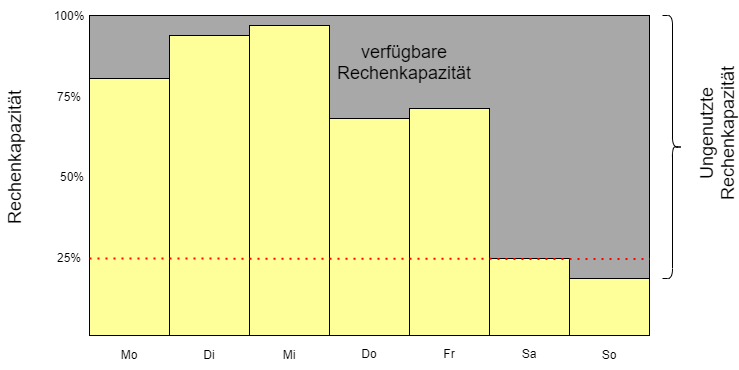
\includegraphics[scale=0.5]{sources/AutoCap Unused Capacity}
    \caption[Ungenutzte Rechenkapazität ohne automatische Skalierung]{}
    \label{fig:AutoSca_Unused_Capacity} Ungenutzte Rechenkapazität ohne automatische Skalierung. \\
    Quelle: Eigene Darstellung mit [fiktiven?] Angaben. 
    %\footnote{\cite{AMZ01}}
  \end{figure}\\
Die gelben Säulen stellen die tägliche genutzte Rechenkapazität dar.
Die graue Zone entspricht ungenutzte Rechenkapazität und beträgt etwa ein Drittel der wöchentlichen Rechnerkapazität.
%Zu erklären: cooldown period and scaling policy.
%Macht die Nutzung von Spor-Instanzen so einfach wie nie zuvor ?
\subsubsection*{Elastic Load Balancing}%https://docs.aws.amazon.com/autoscaling/ec2/userguide/autoscaling-load-balancer.html
[]
\subsubsection{Zeitgesteuerte Skalierung}
%W-Ende für Dev und Beta
\textbf{Nicht produktive Umgebungen}\\
%Auch möglich damit https://aws.amazon.com/de/solutions/implementations/instance-scheduler/
In einem On-Premise-System macht es, wenn überhaupt, einen kleinen Unterschied bei den Kosten, dass Instanzen die ganze Zeit aktiv bleiben. Im Gegensatz dazu ist es bei On-Demand-Zahlungsmodelle sinnvoll Zeiträume zu definieren, in denen Instanzen abgeschaltet werden können, um der Nutzung von AWS-Diensten zu reduzieren. Bei Systemen, die nur tagsüber und unter der Woche in Betrieb sein müssen, kann dies eine Einsparung von zu 67\% bedeuten.  Wenn zum Beispiel Test- und Beta-Umgebungen von Montag bis Freitag von 7 bis 20 Uhr laufen würden.
\begin{figure}[h]
  \centering
  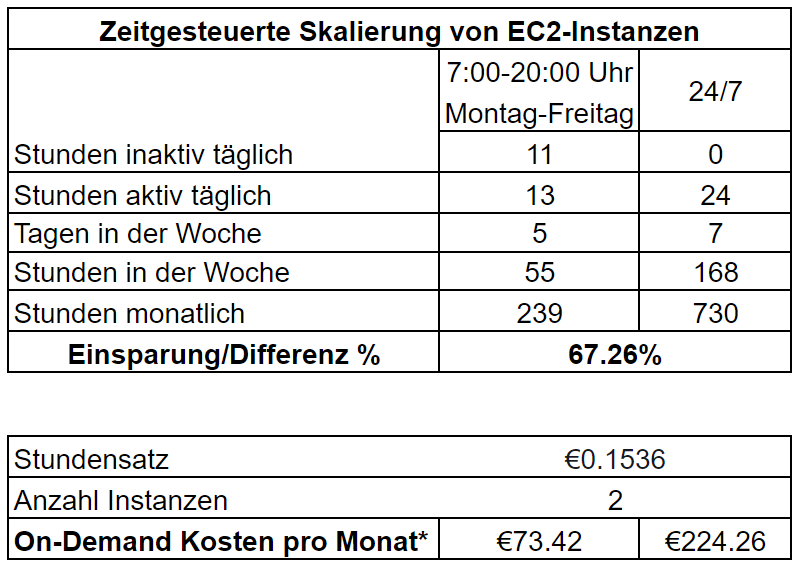
\includegraphics[scale=0.6]{sources/Einsparung_Zeitgesteuerte_Skalierung}
  \caption[Berechnung für ein nicht produktives Umgebung mit Zeitgesteuerte Skalierung]{}
  \label{fig:Einsparung_Zeitgesteuerte_Skalierung} Berechnung für ein nicht-produktive Umgebung mit Zeitgesteuerte Skalierung. \\
  Quelle: Eigene Darstellung. 
  %\footnote{\cite{AMZ01}}
\end{figure}
\\
Der Stundensatz wurde am 23.11.2021 mit dem AWS Pricing Calculator\cite{AMZ17} ermitellt für Linux Instanzen in Frankfurt mit 4vCPUs, 16 GB Arbeitsspeicher und Instanz-Familie t4g.xlarge in On-Demand-Zahlungsmodell.
% Automatisiere das Hoch- und Herunterfahren von Instanzen
% https://www.linkedin.com/learning/monitoring-aws-with-cloudwatch/autoscaling-using-alarms?autoAdvance=true&autoSkip=true&autoplay=true&resume=false&u=79182202
% Grund: weil i.d.R., kein Entwickler 24/7 arbeitet.
% Wie?: mit Tagging, Lambda oder mit Auto Scaling Groups.
%Wann ist es sinnvoll Systeme runterzufahren 
%HIER LESEN {\cite{CCB}, Seite 153}
%Weihnachten und BackFriday
\\\\
\textbf{Produktive Umgebungen}\\
Wenn der Zeitpunkt einer hohen Nachfrage bekannt ist, kann eine Erhöhung der Rechnerkapazität geplant werden, um Überlastungen zu vermeiden. Beispiele für solche Zeiträume sind Cyber-Monday und Black Friday\footnote{\cite{STA5}Wie viel planen Sie am Black Friday / Cyber Monday auszugeben?}. 
[WEITERE ERKLÄRUNG]
%https://de.statista.com/statistik/daten/studie/1076963/umfrage/ausgaben-an-black-friday-und-cyber-monday-in-deutschland/]

\subsubsection{Dynamisches Auto Scaling}
%Intro mit Beispiel
Es kann jedoch zu schnelle und kontinuierliche Änderungen im Verhalten von Applikationen geben, häufig innerhalb von wenige Minuten. Bei solche Szenarien ist sinnvoller, Metriken zur automatischen Anpassung der Skalierung der Rechenkapazität festzulegen. Beispiele für eine veränderte Nutzung von Applikationen finden sich bei Tinder und OkCupid, zwei der größten Dating-Applikationen in den vereinigten staaten. \\
Die \autoref{fig:Use_by_hour_netflix_OkCupid_tinder} zeigt die Nutzungsspitzen bei den genannten Applikationen. Dieses wechselnde Verhalten wirkt sich unmittelbar auf die zu verschiedenen Tageszeiten benötigte Rechenkapazität aus und macht eine dynamische Skalierung der Rechenkapazität erforderlich, wenn das Ziel darin besteht, ungenutzte Cloud-Dienste abzuschalten. Als Konsequenz der Abschaltung von ungenutzten Cloud-Diensten folgt die Reduzierung von Kosten.[Rev]
\begin{figure}[h!]
  \centering
  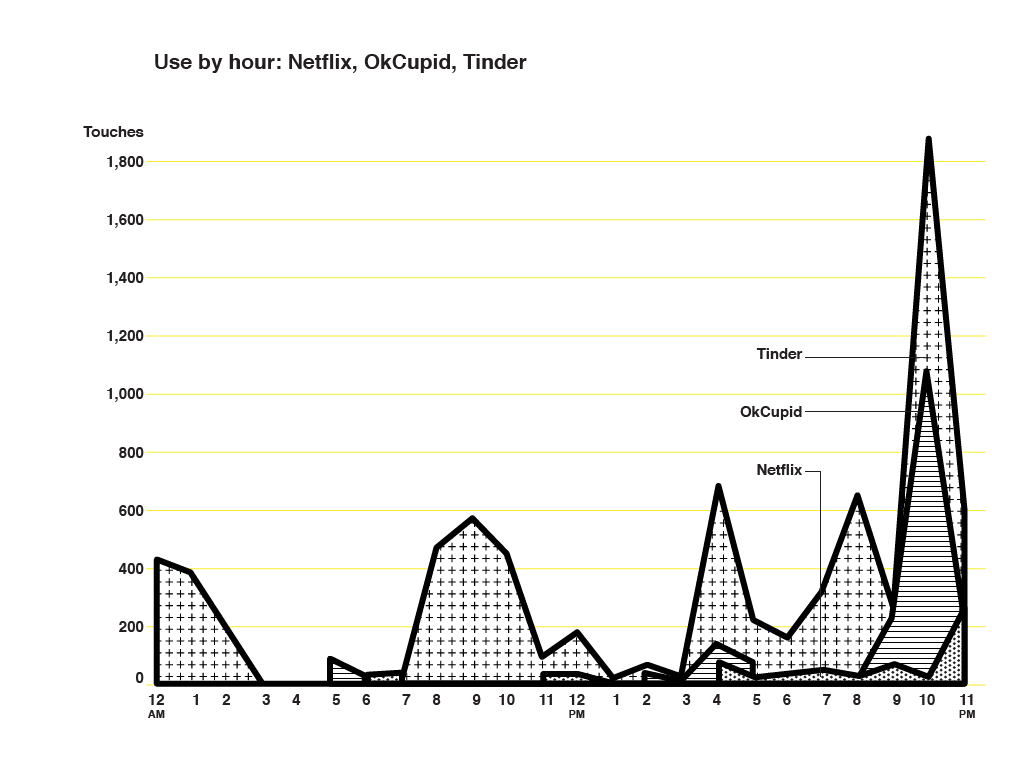
\includegraphics[scale=0.4]{sources/Use_by_hour_netflix_OkCupid_tinder}
  \caption[Nutzung von Tinder, OkCupid und Netflix pro Stunde]{}\label{fig:Use_by_hour_netflix_OkCupid_tinder} Nutzung von Tinder, OkCupid und Netflix pro Stunde.  
  %Quelle: Eigene Darstellung. 
  \footnote{\cite{SCOUT1}}
  \\Mit Touches sind die Anzahl der Klicks, Swipes oder einfachen Interaktionen mit der Applikation gemeint.
\end{figure}
Die für die automatische Skalierung erforderlichen Metriken wurden bereits im Kapitel Überwachungswerkzeuge erwähnt. Eine der Metriken, die von Cloudexperten [TELEFONAT mit Deepak von der Einheit CIS[Cloud Capgemini]]benutzt wird, ist die gesamte CPU-Auslastung. 
Um die CPU-Auslastung als Metrik zu verwenden, werden mindestens zwei Schwellenwerte definiert. Eine für die Erhöhung von Rechenkapazität, Scale-Out genannt und eine für das Verringern von Rechenkapazität bezeichnet als Scale-In.

\subsubsection{Manual Scaling}
%CHECK/23.11\\
Für die Konfiguration einer Auto-Scaling-Gruppe werden die minimale, maximale und gewünschte Anzahl von Instanzen definiert. Wenn aufgrund von Bedingungen, die in der Konfiguration einer Auto-Scaling-Gruppe nicht berücksichtigt wurden mehr Rechenkapazität benötigt wird, ist es möglich, die Rechenkapazität manuell zu steuern. Dies geschieht, ohne dass die aktiven Instanzen unterbrochen werden.

\subsubsection{Predective Scaling}%Voraussagende Skalierung / 
Voraussagende Skalierung oder Predictive Scaling auf Englisch, nutzt maschinelles Lernen, um den Kapazitätsbedarf auf der Grundlage historischer Daten von CloudWatch vorherzusagen. Mit Hilfe der Predictive Scaling kann es die Kapazität vor der erwarteten Auslastung bereitstellen, im Gegensatz zur dynamischen Skalierung, die reaktiv ist. 
Für Instanzen, die viel Zeit für die Initialisierung benötigen kann die Zeit zwischen dem Beginn des Nachfrageanstiegs und der Initialisierung der Instanz vermieden oder verkürzt werden.
[(EIGENES) DIAGRAMM]
Anders als Zeitgesteuerte Skalierung ist es nicht notwendig, die Verhaltensmuster der Anwendungen zu analysieren.
%[SOLLTE DAS ZITIERT WERDEN?]
%https://docs.aws.amazon.com/autoscaling/ec2/userguide/as-dg.pdf#ec2-auto-scaling-predictive-scaling

\subsection{S3 Optimierung}
\subsubsection{Die richtige Speicherklassen wählen}
Um die Speicherkosten zu optimieren, ist es daher notwendig, die richtige Speicherklassen für die jeweilige Applikation wählen. Um die richtige Wahl zu treffen, müssen die Anforderungen der Applikation verstanden werden. Klinische Patientendaten und eine Instagram-Story unterscheiden sich in der Zugriffshäufigkeit auf diese Daten und in der Länge der Aufbewahrungszeit.

Amazon bietet verschiedene Speicherklassen an, die sich im Preis und in der Häufigkeit des Zugriffs auf die Objekte unterscheiden. Objekte sind in Behältern enthalten, die Buckets genannt werden.
[ABB Speicherklasse ->Eigenschaften der Anwendung?]
Wenn Daten über einen längeren Zeitraum gespeichert werden müssen, weil die Anforderungen der Applikation dies vorschreiben oder für den Fall dass, per Gesetz auf die Informationen in der Zukunft zugegriffen werden muss.
%\\
[UMFORMULIEREN]
Zusätzlich, wenn auf die Daten nicht häufig zugegriffen wird, sind Glacier und Glacier Deep Archive passende Speicherklassen. Die Entscheidung ist jedoch nicht immer so einfach und die Umstände können sich schnell ändern. Hinzu kommt, dass nicht alle Daten in einer Applikation immer die gleichen Zugriffsmuster haben. Für solche Fälle ist es möglich, Regeln zu definieren, die Dateien zwischen verschiedenen Speicherklassen abhängig von ihrem Alter übertragen.

\subsubsection{Lebenszyklus-Konfiguration}
[MASSNAHME für...]Eine S3-Lebenszykluskonfiguration oder lifecycle policy beschreibt in einer XML-Datei Regeln und Aktionen für die Manipulation von Objekten.
Aktionen wie das Verschieben von Objekten verursachen Kosten. Ein Beispiel von diesen Kosten und mögliche Einsparungen werden in \autoref{fig:Kostenvergleich_Nutzung_unt_Speicherklassen} für die Berechnung der Speicherkosten verwendet.
\\
%Beim Verschieben nach S3 Intelligent-Tiering, S3 Standard – Infrequent Access und S3 One Zone – Infrequent Access: %\$0.01\\
%S3 Glacier: \$0.036\\
%S3 Glacier Deep Archiv: \$0.06\\
%Datenabfrage am 24.11.2
%{\cite{AMZ09}}
%\\
Um konkretere Regeln zu zu definieren, ist es möglich Tags zu verwenden und somit eine Unterscheidung zwischen Objekten mit verschiedenen Tags zu treffen.
Es ist zum Beispiel möglich, alle Objekte mit dem Tag: Dev nach 45 Tagen nach Standard Infrequent Access und nach 120 Tagen nach S3 Glacier zu verschieben.

\begin{lstlisting}
  <LifecycleConfiguration>
  <Rule>
    <ID>example-id</ID>
    
 <Filter>
      <Tag>
         <Key>key</Key>
         <Value>Dev</Value>
      </Tag>
</Filter>

    <Status>Enabled</Status>
    <Transition>
      <Days>45</Days>
      <StorageClass>STANDARD_IA</StorageClass>
    </Transition>
    <Transition>
      <Days>120</Days>
      <StorageClass>GLACIER</StorageClass>
    </Transition>
    <Expiration>
      <Days>365</Days>
    </Expiration>
  </Rule>
</LifecycleConfiguration>

Angepasster Code auf Basis der Beispiele auf Seite 701 in 
Amazon Simple Storage Service - User Guide, 
\end{lstlisting}
\footnote{\cite{AMZ18}, Seite 701}
Zur Veranschaulichung (der gezeigten Informationen[OHNE ODER DAMIT?]) wird davon ausgegangen, dass ein Sicherheitsunternehmen, das Sicherheitsvideos speichern muss, im Durchschnitt 120 TB an Videos speichern muss. Viele von ihnen werden mindestens 5 Jahre lang aufbewahrt, falls sie vor Gericht als Beweismittel dienen. Ungefähr 50\% der Videos werden mindestens einmal im Monat überprüft und müssen laut Gesetz sofort zugänglich sein. Die Software des Unternehmens speichert die Videos in S3-Buckets und hat eine durchschnittliche Größe von 3,4 GB.

Im Folgenden werden die Speicherkosten für ein Szenario berechnet, bei dem nur S3 Standard verwendet wird. Als nächstes wird die Kombination von S3 Standard Infrequent Access, S3 Glacier und S3 Standard für ein Szenario betrachtet, in dem die Dateien je nach Alter verschoben werden. Im letzten Szenario müssen die Kosten für den Übergang[RICHTIGES WORT?] zwischen Speicherklassen berücksichtigt werden.
\\
Zur Vereinfachung der Berechnung wird angenommen, dass 20\% der Dateien in S3 Standard Infrequent Access und 30\% in S3 Glacier gespeichert werden.
\\
\begin{figure}[h!]
  \centering
  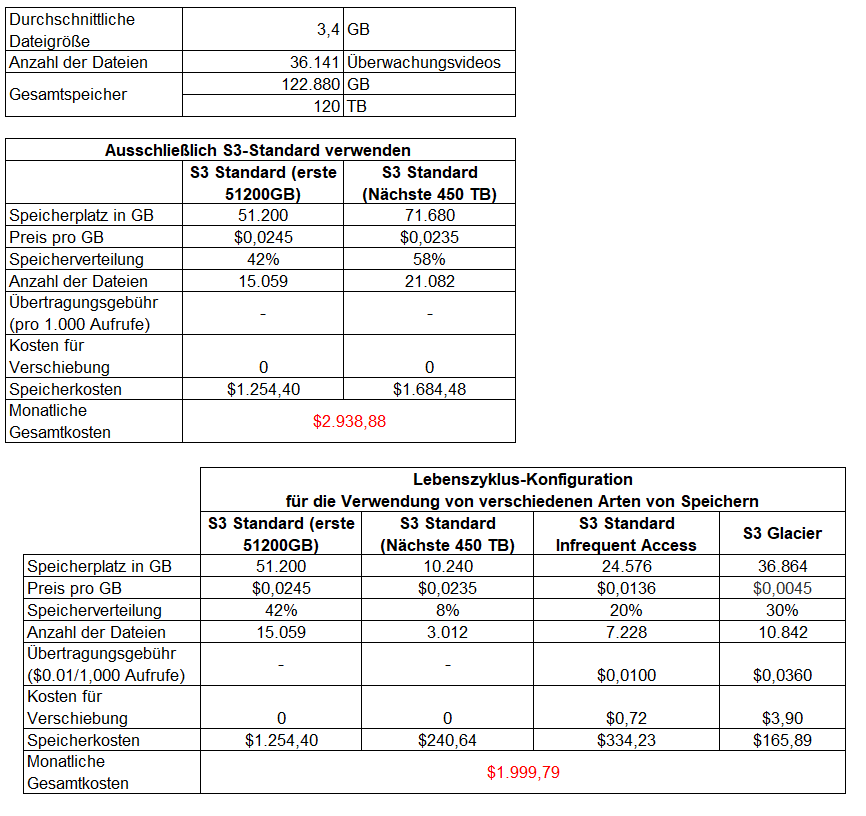
\includegraphics[scale=0.75]{sources/Kostenvergleich_Nutzung_unt_Speicherklassen}
  \caption[Kostenvergleich durch Nutzung von unterschiedlichen Speicherklassen]{}\label{fig:Kostenvergleich_Nutzung_unt_Speicherklassen} 
  Kostenvergleich durch Nutzung von unterschiedlichen Speicherklassen.  \\
  Quelle: Eigene Darstellung. S3 Stundensätze: \footnote{\cite{AMZ09}}\\
Der Punkt wurde als Dezimaltrennzeichen und das Komma als Tausendertrennzeichen verwendet.
\end{figure}
%\\
Bei der Berechnung wurden die Kosten für das Verschieben von Dateien zwischen Speicherklassen berücksichtigt. 
Anhand der Berechnungen lässt sich erkennen, dass ein Einsparungspotenzial von rund 1.000 Dollar pro Monat besteht, indem die notwendigen Regeln aufgestellt werden, um einen Teil der Dateien in anderen Speicherklassen zu verschieben, welche niedrigere Preise bieten.

%WICHTIG IST DIE GRÖSSE MEINE DATEIEN UND DIE ANZAHL.
%weil SO WERDEN DIE PREISE FÜR VERSCHIEBUNG BERECHNET.
%(Object size distribution )
\newpage
\subsubsection{Intelligent-Tiering}
Intelligent-Tiering verschiebt Dateien auf der Grundlage von Zugriffsmustern. Diese Speicherklasse ist ideal für Daten mit wechselnden oder unbekannten Zugriffsmustern. 
Wie die Senior Product Manager für S3 Ruhi Dang erklärt, einige Unternehmen haben weder die Zeit noch die finanziellen Möglichkeiten, eine Person einzustellen, die ihre Daten sortiert und in die richtige Speicherklasse einordnet. Intelligent Auto Tiering ist eine attraktive Lösung für Unternehmen, die jährlich weniger als \$100,000 für Speicher ausgeben \footnote{\cite{AMZ16},AWS re:Invent 2019: Guidelines and design patterns for optimizing cost in Amazon S3. Minute: 21:12}.
%Ach von Jessie Felix gesagt https://www.youtube.com/watch?v=IOT41L_adSw
%\\\\
\autoref{fig:S3_IntLifeCycle} zeigt, wie die Dateien in Abhängigkeit davon, ob auf sie zugegriffen wurde oder nicht, verschieben werden. 
\begin{figure}[h!]
  \centering
  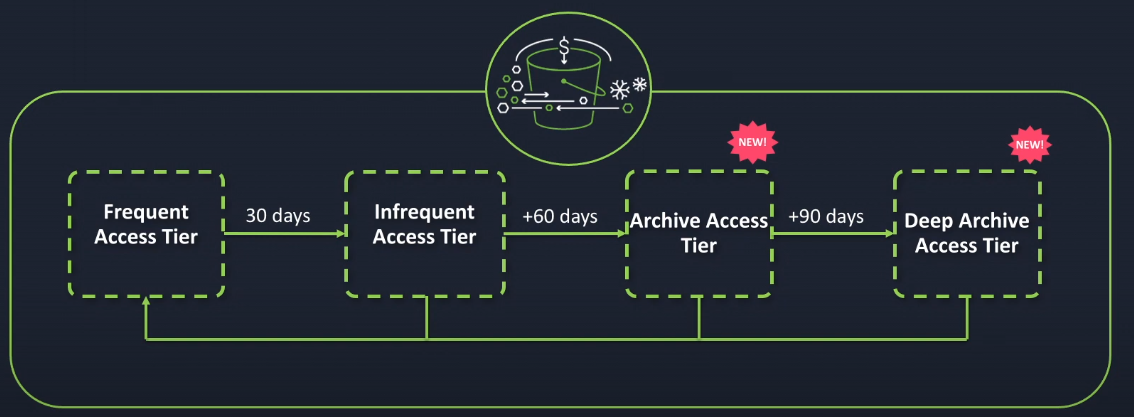
\includegraphics[scale=0.7]{sources/S3_IntLifeCycle}
  \caption[Funktionsweise von Intelligent-Tiering]{}\label{fig:S3_IntLifeCycle} Funktionsweise von Intelligent-Tiering\\
  Quelle: Eigene Darstellung
  %{\cite{SCOUT1}}
\end{figure}
Wird ein Datei zu einem späteren Zeitpunkt aus der Ebene der seltenen Zugriffe aufgerufen, wird es automatisch in eine Speicherklasse der häufigen Zugriffe zurückversetzt.















%COMMENTS
\begin{comment}
\subsubsection{Automatisierung mit Lambda Funktionen}
Grund: einmal programmiert, funktioniert es für immer.
\\(To-Do:) Möglichkeiten untersuchen, bewerten und die passende Auswählen.

%Limitierung 
%Quotas setzen? erweitern oder reduzieren / benachrichtigen aber auch eine Aktion durchführen 

%Lambda

AWS Lambda is a compute service. You can use it to run code without provisioning or managing servers. Lambda runs your code on a high-availability compute infrastructure. It operates and maintains all of the compute resources, including server and operating system maintenance, capacity provisioning and automatic scaling, code monitoring, and logging. With Lambda, you can run code for almost any type of application or backend service. 

Some benefits of using Lambda include the following:

You can run code without provisioning or maintaining servers.
It initiates functions for you in response to events.
It scales automatically.
It provides built-in code monitoring and logging via Amazon CloudWatch.
\end{comment}

%Data Pipeline

%Economic Performance?
%QUEUES

%NEVER forget your availability requirements, trying to optimize, first availability THEN cost...
%Do not use your DB for saving BLOB

%\subsection{VERKAUFE DEINE Ungenutzte Kapazität in RI Marketplace}

%Kombination
%https://spot.io/blog/effective-utilization-of-aws-savings-plans-and-ec2-spot-instances/#a1
%https://www.youtube.com/watch?v=X_7pnzPlESs

 